\chapter{Signal Processing Basics}
\label{chap:appendixsignalprocessing}
The aim of this appendix chapter is to provide the reader some basic knowledge in signal processing, Fourier transformations and related mathematical concepts. It is recommended to understand all the mathematical concepts mentioned in this appendix chapter in order to be able to follow all derivation steps performed during this thesis. 

\section{Signals in Signal Processing}
A \emph{signal} is a function that conveys information about the behavior or attributes of some phenomenon. In the physical world, any quantity that exhibits variation in time or in space (such as an image) is potentially a signal. Such a signal might carry information about the state of a physical system, or might convey a message between observers. \\

\section{Fourier Transformation}
The \emph{Fourier transform} is a mathematical tool which allows to transform a given function or rather a given signal from defined over a time- (or spatial-) domain into its corresponding frequency-domain. \\

The Fourier transform is an important image processing tool which is used to decompose an image into its sine and cosine components. The output of such a Fourier transformation represents the image in its frequency domain. On the other hand, the input image is usually in the spatial domain. In the frequency domain of the Fourier transformation of an image, each point represents a particular frequency contained in the spatial domain image. \\

Next let us consider some mathematical definitions of Fourier transformations. Let $f$ be a measurable function over $\mathds{R}^n$. Then, its continuous \emph{Fourier Transformation} (\textbf{FT}) $\mathcal{F}\{f\}$$\footnote{Note that for simplification purposes we omit some constant factors in our definitions for the Fourier transformation.}$ is defined as:
 
\begin{equation}
  \mathcal{F}_{FT}\{f\}(w) = \int_{\mathds{R}^n} f(x)e^{-iwt} dt
  \label{eq:cft}
\end{equation}

whereas its \emph{inverse transformation} is defined like the following which allows us to obtain back the original signal:

\begin{equation}
  \mathcal{F}_{FT}^{-1}\{f\}(w) = \int_{\mathds{R}} \mathcal{F}\{w\}e^{iwt} dt
  \label{eq:icft}
\end{equation}

Where $w$ usually denotes the \emph{angular frequency}, which is equal to 
\begin{equation}
  w = \frac{2 \pi}{T} = 2 \pi v_f 
\end{equation}

Furthermore denotes $T$ the \emph{period} of the spectrum and $v_f$ is its corresponding \emph{frequency}. Notice that the definitions we use for the Fourier transformation correspond to the definition physicist and mathematicians typically use. However, there are other possibilities to define the Fourier transformation such as the definition used in electrical engineering. For further information about this kind of Fourier transformation please have a look at section $\ref{sec:electricalengeneeringftconvention}$. \\

By using Fourier analysis$\footnote{Fourier analysis is the technique to approximate a function by a sums of simpler trigonometric functions.}$ we can derive \emph{Discrete Time Fourier Transform} (\textbf{DTFT}). The DTFT operates on a discrete function. Such an input function is often created by digitally sampling a continuous function. The DTFT generates a continuous and periodic signal in the frequency domain. This operator is defined as the following:

\begin{equation}
  \mathcal{F}_{DTFT}\{f\}(w) = \sum_{-\infty}^{\infty} f(x) e^{-iwk}
  \label{eq:dtft}
\end{equation}

Note that the DTFT is not practically suitable for digital signal processing since there a signal can be measured only in a finite number of points. Thus, by discretize its frequency domain we get the \emph{Discrete Fourier Transformation} (\textbf{DFT}) of the input signal:

\begin{equation}
  \mathcal{F}_{DFT}\{f\}(w) = \sum_{n=0}^{N-1} f(x) e^{-iw_{n}k}
  \label{eq:dft}
\end{equation}

Where the angular frequency $w_n$ is defined as the following:

\begin{equation}
  w_n = \frac{2\pi n}{N} 
\end{equation}
\noindent
and $N$ is the number of samples within an equidistant period sampling. \\

Any continuous function $f(t)$ can be expressed as a series of sines and cosines. This representation is called the \emph{Fourier Series} (\textbf{FS}) of $f(t)$.
\begin{equation}
  f(t) = \frac{1}{2}a_0 + \sum_{n=1}^{\infty} a_n cos(nt) + \sum_{n=1}^{\infty} b_n cos(nt)
  \label{eq:dfs}
\end{equation}

where

\begin{align}
    a_0 = \int_{-\pi}^{\pi} f(t) dt \nonumber \\
    a_n = \frac{1}{\pi}\int_{-\pi}^{\pi} f(t) cos(nt) dt \nonumber \\
    b_n = \frac{1}{\pi}\int_{-\pi}^{\pi} f(t) sin(nt) dt
\end{align}

Figure $\ref{fig:contdiscft}$ illustrated the relationships between the different Fourier transformation types.

\begin{figure}[H]
  \centering
  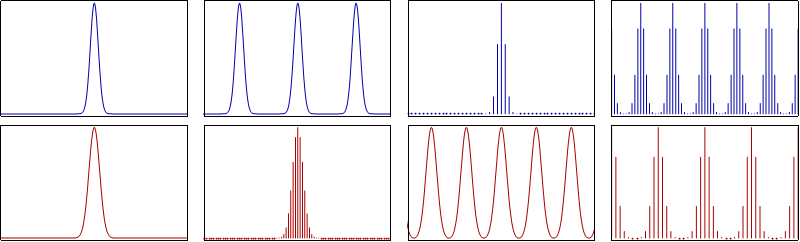
\includegraphics[scale=0.5]{background/dcft.png}
  \caption[Relationships between of Different Fourier Transformations]{Relationship$\footnotemark$ between the continuous Fourier transform and the discrete Fourier transform: Left column: A continuous function (top) and its Fourier transform $\ref{eq:cft}$ (bottom). Center-left column: Periodic summation of the original function (top). Fourier transform (bottom) is zero except at discrete points. The inverse transform is a sum of sinusoids called Fourier series $\ref{eq:dfs}$. Center-right column: Original function is discretized (multiplied by a Dirac comb) (top). Its Fourier transform (bottom) is a periodic summation (DTFT) of the original transform. Right column: The DFT $\ref{eq:dft}$ (bottom) computes discrete samples of the continuous DTFT $\ref{eq:dtft}$. The inverse DFT (top) is a periodic summation of the original samples.}
\label{fig:contdiscft}
\end{figure}
\footnotetext{This image has been taken from \texttt{http://en.wikipedia.org/wiki/Discrete\textunderscore Fourier\textunderscore transform}}

Table $\ref{tab:ftoperatorsdependencies}$ represents a summary of the different Fourier transformation types. It tells the reader which Fourier Operator take what kind of input signal and what properties its corresponding output signal will have.

\begin{table}[H]
    \begin{tabular}{l|l|l}
    \hline
    Spatial signal $f(t)$ is & Operator & Transformed frequency signal $\hat{f}(\omega)$ is\\
    \hline
    continuous and periodic in $t$ & $FS$ see Eq. $\ref{eq:dfs}$ & only discrete in $\omega$ \\
    only continuous in $t$ & $FT$ see Eq. $\ref{eq:cft}$ & only continuous in $\omega$\\
    only discrete in $t$ & $DTFT$ see Eq. $\ref{eq:dtft}$ & continuous and periodic in $\omega$\\
    discrete and periodic in $t$ & $DFT$ see Eq.$\ref{eq:dft}$ & discrete and periodic in $\omega$\\
    \hline
    \end{tabular}
\caption[Fourier Transform Mapping]{Fourier operator to apply for a given spatial input signal and the properties of its resulting output signal in frequency space}
\label{tab:ftoperatorsdependencies}
\end{table}

\section{The Convolution Operator}
In signal processing we use the \emph{convolution} operator mostly for performing any kind of filtering operations applied on given signals.
Mathematically, this operator is a form of combining two signals (i.e. weighting one signal by the other). The output of a convolution is always a continuous function. The convolution $f*g$ of two functions $f$, $g$$\colon \mathds{R}^n \to \mathds{C} $ is defined as:  
\begin{equation}
  \mathcal (f*g)(t) = \int_{\mathds{R}^n} f(t)g(t-x) dx
  \label{eq:convolution}
\end{equation}

Note that the Fourier transform of the convolution of two functions is equal to the product of their Fourier transforms. In other words a convolution in a spatial domain is equivalent to a multiplication in frequency domain. Therefore, the inverse Fourier transform of the product of two Fourier transforms is equal to the convolution of the two inverse Fourier transforms. \\

\section{Taylor Series}
In mathematics we use \emph{Taylor series} in order to approximate functions by a series of its derivatives. Conceptually, a Taylor series is mathematical concept which allows to represent a function by a certain infinite series.  \\

The Taylor series $\mathcal T$ of an infinitely differentiable real or complex valued function $f(x)$ evaluated on a point $a$ is equal to the following power series:

\begin{equation}
  \mathcal T(f;a)(x) = \sum_{n=0}^{\infty} \frac{f^{n}(a)}{n!}(x-a)^n
  \label{eq:deftaylor}
\end{equation}